%%
%% This is file `sample-sigconf.tex',
%% generated with the docstrip utility.
%%
%% The original source files were:
%%
%% samples.dtx  (with options: `sigconf')
%%
%% IMPORTANT NOTICE:
%%
%% For the copyright see the source file.
%%
%% Any modified versions of this file must be renamed
%% with new filenames distinct from sample-sigconf.tex.
%%
%% For distribution of the original source see the terms
%% for copying and modification in the file samples.dtx.
%%
%% This generated file may be distributed as long as the
%% original source files, as listed above, are part of the
%% same distribution. (The sources need not necessarily be
%% in the same archive or directory.)
%%
%% Commands for TeXCount
%TC:macro \cite [option:text,text]
%TC:macro \citep [option:text,text]
%TC:macro \citet [option:text,text]
%TC:envir table 0 1
%TC:envir table* 0 1
%TC:envir tabular [ignore] word
%TC:envir displaymath 0 word
%TC:envir math 0 word
%TC:envir comment 0 0
%%
%%
%% The first command in your LaTeX source must be the \documentclass command.
\documentclass[sigconf]{acmart}
\usepackage{afterpage}
\usepackage{float}
%% NOTE that a single column version is required for
%% submission and peer review. This can be done by changing
%% the \doucmentclass[...]{acmart} in this template to
%% \documentclass[manuscript,screen]{acmart}
%%
%% To ensure 100% compatibility, please check the white list of
%% approved LaTeX packages to be used with the Master Article Template at
%% https://www.acm.org/publications/taps/whitelist-of-latex-packages
%% before creating your document. The white list page provides
%% information on how to submit additional LaTeX packages for
%% review and adoption.
%% Fonts used in the template cannot be substituted; margin
%% adjustments are not allowed.

%%
%% \BibTeX command to typeset BibTeX logo in the docs
\AtBeginDocument{%
  \providecommand\BibTeX{{%
    \normalfont B\kern-0.5em{\scshape i\kern-0.25em b}\kern-0.8em\TeX}}}

%% Rights management information.  This information is sent to you
%% when you complete the rights form.  These commands have SAMPLE
%% values in them; it is your responsibility as an author to replace
%% the commands and values with those provided to you when you
%% complete the rights form.
\setcopyright{acmcopyright}
\copyrightyear{2023}
\acmYear{2023}
\acmDOI{XXXXXXX.XXXXXXX}

%% These commands are for a PROCEEDINGS abstract or paper.
\acmConference[WSDM '24]{The 17th ACM International Conference on Web Search and Data Mining}{March 04--08,2024}{Mérida, MX}
%
%  Uncomment \acmBooktitle if th title of the proceedings is different
%  from ``Proceedings of ...''!
%
%\acmBooktitle{Woodstock '18: ACM Symposium on Neural Gaze Detection,
%  June 03--05, 2018, Woodstock, NY}
\acmPrice{15.00}
\acmISBN{978-1-4503-XXXX-X/18/06}


%%
%% Submission ID.
%% Use this when submitting an article to a sponsored event. You'll
%% receive a unique submission ID from the organizers
%% of the event, and this ID should be used as the parameter to this command.
%%\acmSubmissionID{123-A56-BU3}

%%
%% For managing citations, it is recommended to use bibliography
%% files in BibTeX format.
%%
%% You can then either use BibTeX with the ACM-Reference-Format style,
%% or BibLaTeX with the acmnumeric or acmauthoryear sytles, that include
%% support for advanced citation of software artefact from the
%% biblatex-software package, also separately available on CTAN.
%%
%% Look at the sample-*-biblatex.tex files for templates showcasing
%% the biblatex styles.
%%

%%
%% The majority of ACM publications use numbered citations and
%% references.  The command \citestyle{authoryear} switches to the
%% "author year" style.
%%
%% If you are preparing content for an event
%% sponsored by ACM SIGGRAPH, you must use the "author year" style of
%% citations and references.
%% Uncommenting
%% the next command will enable that style.
%%\citestyle{acmauthoryear}

%%
%% end of the preamble, start of the body of the document source.
\usepackage{multirow}
\usepackage{booktabs}
\begin{document}

%%
%% The "title" command has an optional parameter,
%% allowing the author to define a "short title" to be used in page headers.
\title{Future Timelines: Extraction and Visualization of Future-related Content  From News Articles}

%%
%% The "author" command and its associated commands are used to define
%% the authors and their affiliations.
%% Of note is the shared affiliation of the first two authors, and the
%% "authornote" and "authornotemark" commands
%% used to denote shared contribution to the research.
\author{Juwal Regev}
\email{juwal.regev@student.uibk.ac.at}
\orcid{1234-5678-9012}
\affiliation{%
  \institution{University of Innsbruck}
  \city{Innsbruck}
  \country{Austria}
}

\author{Adam Jatowt}
\affiliation{%
  \institution{University of Innsbruck}
  \city{Innsbruck}
  \country{Austria}}
\email{adam.jatowt@uibk.ac.at}

\author{Michael Färber}
\affiliation{%
  \institution{Karlsruhe Institute of Technology}
  \city{Karlsruhe}
  \country{Germany}}
\email{michael.faerber@kit.edu}


%%
%% By default, the full list of authors will be used in the page
%% headers. Often, this list is too long, and will overlap
%% other information printed in the page headers. This command allows
%% the author to define a more concise list
%% of authors' names for this purpose.
%% \renewcommand{\shortauthors}{Trovato and Tobin, et al.}

%%
%% The abstract is a short summary of the work to be presented in the
%% article.
\begin{abstract}
In today's rapidly evolving world, maintaining a comprehensive overview of the future landscape is essential for staying competitive and making informed decisions. However, given the overwhelming volume of daily news, manually obtaining a thorough overview of an entity's future prospects is quite challenging. To address this, we present a system that is designed to automatically extract future-related information of a queried entity from news articles. Our approach involves fine-tuning a language model on a novel multi-source dataset consisting of 6,800 annotated sentences to identify future-related sentences. We use topic modeling to extract the main topics from the data, which, along with their contents, are subsequently ranked by relevance. A temporal tagger is utilized to detect temporal expressions and map them to specific dates. This enables the sentences to be presented on an interactive timeline. User evaluations have shown favorable feedback on the timelines and summaries our system produces.
\end{abstract}

%%
%% The code below is generated by the tool at http://dl.acm.org/ccs.cfm.
%% Please copy and paste the code instead of the example below.
%%
\begin{CCSXML}
<ccs2012>
   <concept>
       <concept_id>10002951.10003317.10003338.10003341</concept_id>
       <concept_desc>Information systems~Language models</concept_desc>
       <concept_significance>500</concept_significance>
       </concept>
   <concept>
       <concept_id>10002951.10003317.10003318.10003320</concept_id>
       <concept_desc>Information systems~Document topic models</concept_desc>
       <concept_significance>500</concept_significance>
       </concept>
   <concept>
       <concept_id>10010147.10010178.10010179.10003352</concept_id>
       <concept_desc>Computing methodologies~Information extraction</concept_desc>
       <concept_significance>500</concept_significance>
       </concept>
 </ccs2012>
\end{CCSXML}

\ccsdesc[500]{Information systems~Language models}
\ccsdesc[500]{Information systems~Document topic models}
\ccsdesc[500]{Computing methodologies~Information extraction}
%%
%% Keywords. The author(s) should pick words that accurately describe
%% the work being presented. Separate the keywords with commas.
\keywords{Future-related Content Extraction, Sentence Classification, Topic Modeling, Time-Tagging, Timeline Generation, Natural Language Processing}

%% A "teaser" image appears between the author and affiliation
%% information and the body of the document, and typically spans the
%% page.
%% \begin{teaserfigure}
%%  \includegraphics[width=\textwidth]{sampleteaser}
%%  \caption{Seattle Mariners at Spring Training, 2010.}
%%  \Description{Enjoying the baseball game from the third-base
%%  seats. Ichiro Suzuki preparing to bat.}
%%  \label{fig:teaser}
%% \end{teaserfigure}

%% \received{20 February 2007}
%% \received[revised]{12 March 2009}
%% \received[accepted]{5 June 2009}

%%
%% This command processes the author and affiliation and title
%% information and builds the first part of the formatted document.
\maketitle

\newpage

\section{Introduction}
A vast amount of news articles is published on the web every single day. A significant amount of those articles contains information that is predictive or related to future events. Extracting and analyzing such information regarding a specific entity would offer a comprehensive overview of its future prospects.

\noindent However doing this manually is not feasible as one would have to sift through the articles line by line, identifying nuanced references to the future. Furthermore, this would have to be done regularly so as to always have the most up-to-date information. Thus, it is clear that an automated system, capable of extracting, processing and visualizing this information is needed. This system would be beneficial in a variety of different fields. From analyzing predictions related to stock market movements, monitoring corporate developments as well as gaining insights into market trends and emerging technologies, the potential applications are limitless.

\noindent To address this problem, we present a system specifically designed for extracting, summarizing, ranking and visualizing future-related content within news collections. The process is initiated by a user providing an entity, whose future should be explored. The system then downloads and preprocesses thousands of news articles related to the provided entity. In the next step, a neural network classifier is employed to classify sentences as either being future-related or not. Following classification, these sentences are organized into distinct topics, which are then presented to the user in a segmented manner. Additionally, the topics are labeled with representative keywords that provide insight into the content of each cluster. To provide an even better overview, we incorporate a temporal perspective into the presentation of the results. We do this by analyzing the sentences for temporal expressions, extracting and normalizing them to a date and then mapping the sentences, ranked by their relevance, onto a timeline.

\noindent In the following, we will delve into the system's architecture, providing implementation details, explaining the user interface and presenting the findings of a user study conducted to assess the system's result quality.

\afterpage{%
  \begin{figure*}[t]
    \centering
    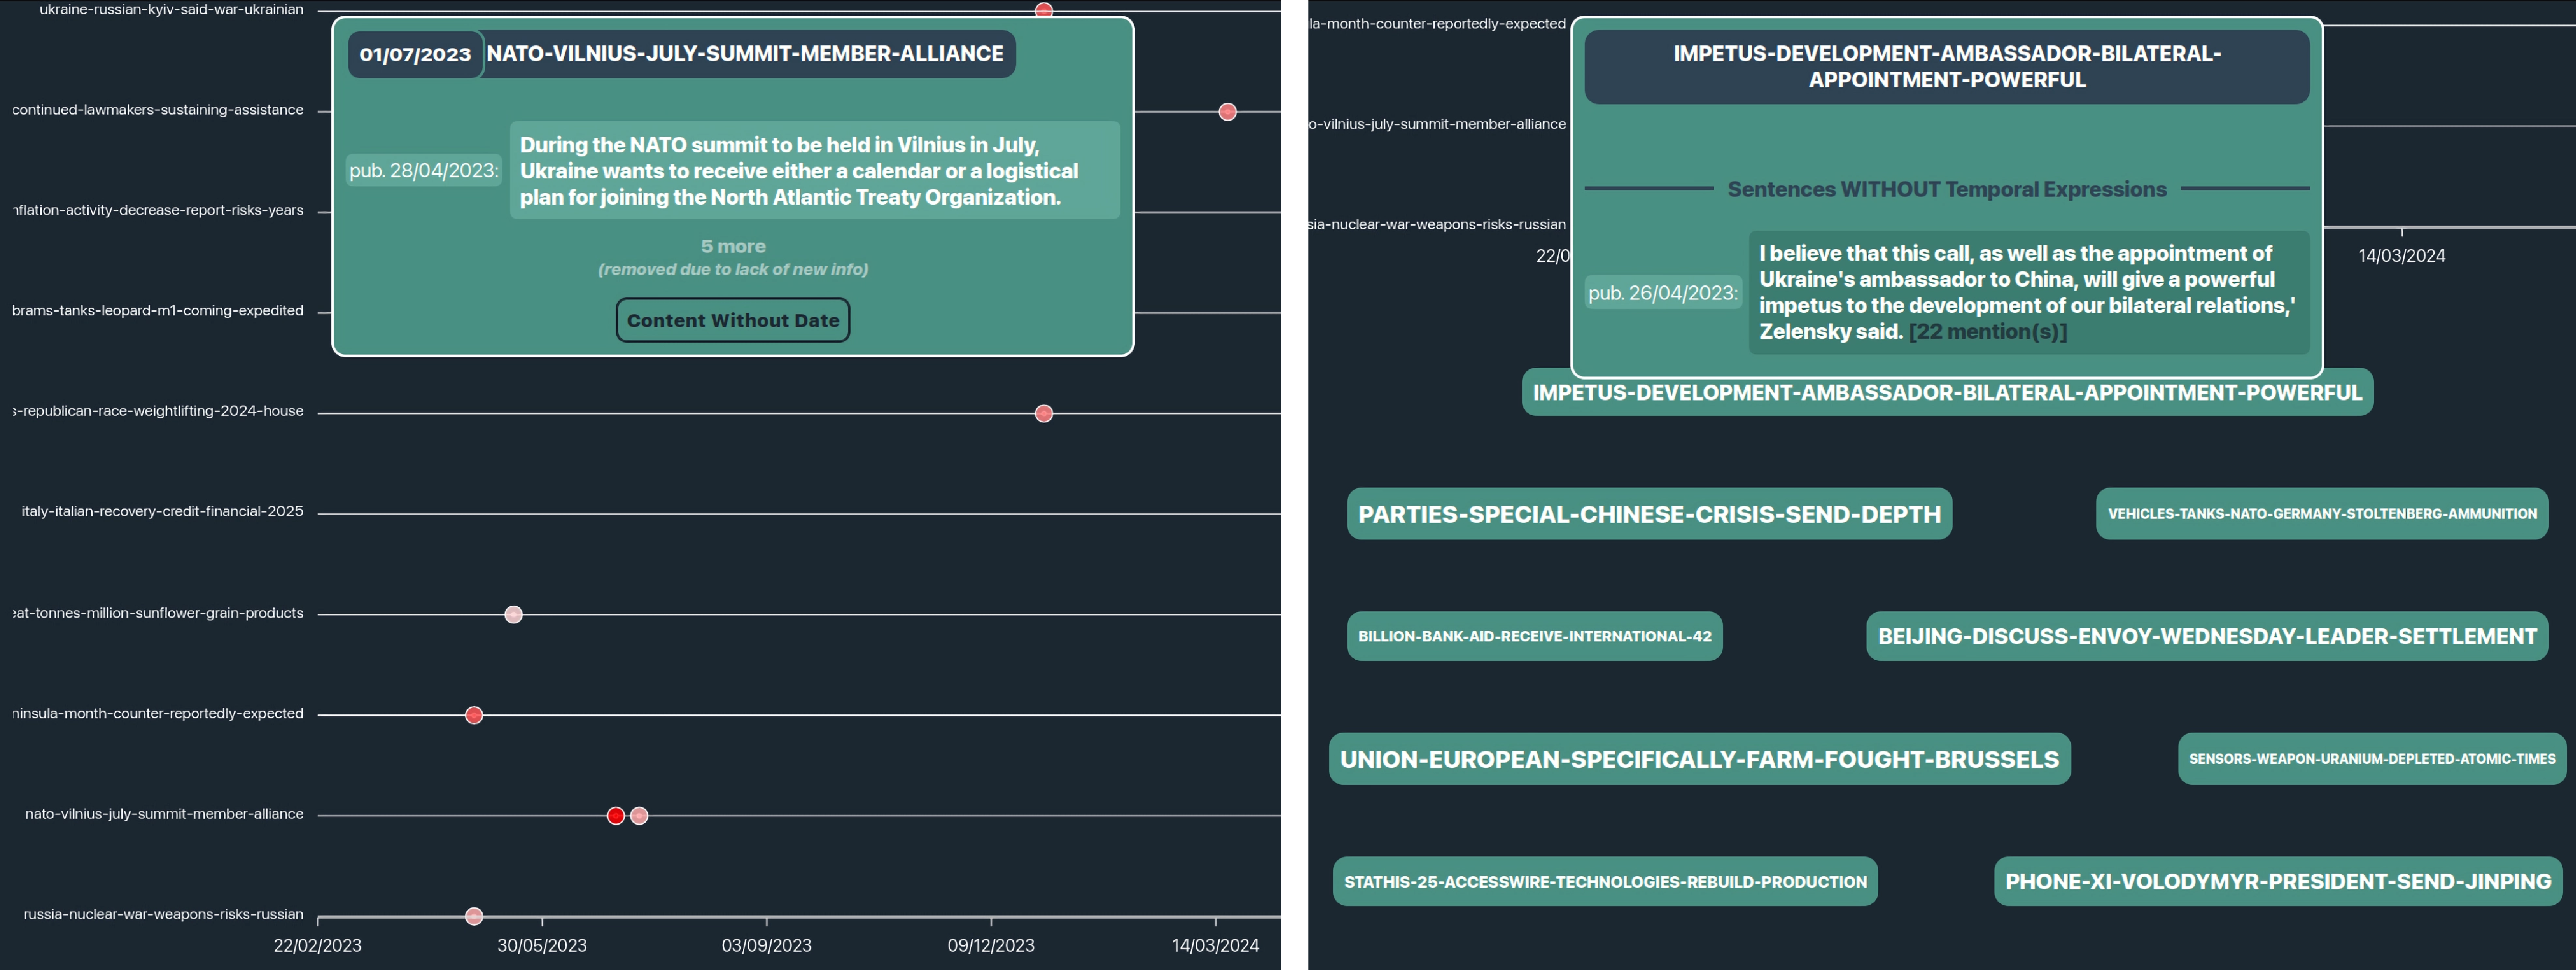
\includegraphics[width=\textwidth]{img/comb.pdf}
    \caption{Visualization of the system's key components: (left) The interactive timeline featuring an open tooltip section, and (right) the Word Cloud also with an open tooltip section.}
    \label{fig:ui}
  \end{figure*}
}



\section{Related Work}
Automatic identification and extraction of future-related information from text has been researched for decades. Baeza-Yates \cite{BaezaYatesSearchingTF} first formalized the concept of "future retrieval". Early methods relied on time-taggers and predefined temporal expressions to extract data, but this resulted in limited diversity \cite{chronoseeker, supportingAnalysis, analyzingCollective, rankingRelated, extractingCollective}. Data was analyzed for unique properties \cite{improvingRetrieval} to create features for classifier training \cite{computationalExploration}.
For example, one study uses morphosemantic patterns as features \cite{automaticExtraction}, while another classifies clauses using features like POS tags and word co-occurrences to determine if a sentence refers to the future \cite{extractingPredictive}. Some systems also predict future events using past data \cite{miningTheWeb, predictingTheNews}.
In Timeline Summarization, content is clustered and ranked to form a timeline. Techniques involve using TF-IDF-vectors or SBERT embeddings \cite{sbert} to represent sentences, and methods like Affinity Propagation \cite{abstractiveTimeline, multiTimeline} and Markov Clustering \cite{stateOfTheArtTimeline} for clustering. Sentence rankings inside of a topic or event often depend on the similarity to a centroid sentence \cite{stateOfTheArtTimeline} or on metrics like date-importance and informativeness \cite{abstractiveTimeline}.



\section{System}
In the following sections, we will introduce our publicly available\footnote{\url{https://github.com/regevson/chronicle2050/}} dataset and system and explore each of its components in depth, gaining a detailed understanding of the overall workflow and examining implementation details.

\subsection{Dataset}
As already mentioned, our approach to data gathering differs from traditional methods. Earlier strategies have frequently relied on extracting data using temporal expressions. However, this approach has its limitations. Predictions can often be intricate, lacking explicit dates or simple temporal cues.
To address this, our dataset incorporates a rich variety of 6,800 manually labeled sentences. They have been collected from different sources without relying on specific queries, and therefore they exhibit unique lexical and structural features and contain a diverse set of topics. This enables our classifier to identify future-related content that does not contain standard temporal expressions hinting at future references.
Table \ref{tab:dataset} provides a breakdown of our data sources.

\vspace*{-0.1cm}

\begin{table}[h]
  \begin{tabular}{lccc}
    \toprule
    \multirow{2}{*}{\textbf{Sources}} & \multirow{2}{*}{\textbf{Positives}} & \multirow{2}{*}{\textbf{Negatives}} & \textbf{Sentences without} \\
    & & & \textbf{temporal expressions (\%)} \\
    \midrule
    Longbets & 448 & 0 & 20 \\
    Horizons & 51 & 62 & 84 \\
    ChatGPT & 305 & 305 & 70 \\
    News & 2501 & 3128 & 39 \\
    \bottomrule
    \textbf{Total} & \textbf{3305} & \textbf{3495} & \textbf{41} \\
  \bottomrule
  \end{tabular}
  \caption{Data Source Analysis: Count of Future-Related (Positive) vs. Non-Future-Related (Negative) Sentences, along with Percentage Free from Temporal Expressions.}
  \label{tab:dataset}
\end{table}


\vspace*{-0.6cm}

\textit{Longbets}\footnote{\url{https://longbets.org/}} is a platform that enables users to share and bet on predictions. In contrast, \textit{Horizons}\footnote{\url{https://radar.envisioning.io/horizons/}} is more focused on emerging technologies. The \textit{News} sentences were extracted from New York Times\footnote{\url{https://www.nytimes.com/}} articles. \textit{ChatGPT}\footnote{\url{https://chat.openai.com/}} was used for its capability to generate highly specific data. Using prompts like \textit{"Generate 50 sentences about various topics that contain future related information. You should use words like ’could, ’may’, ’might’, ..."}, we were able to obtain highly specific and tailored training data.


\subsection{System Overview}
We will now take a closer look at our system's five main components: 1) Data Retrieval and Preprocessing, 2) Classification, 3) Topic Modeling, 4) Postprocessing, 5) Time-Tagging. A visualization of the workflow can be seen in Figure \ref{fig:archi}.

\subsubsection{Fetching and Preprocessing}
To initiate the process, the user has to provide a query to the system, which can take the form of a topic, an entity, or any other input whose future should be analyzed. The user has the option to choose the number of articles that should be downloaded, as well as the time frame from which these articles should be fetched. Once the articles are downloaded, they are split up into their constituent sentences. These sentences subsequently undergo preprocessing to prepare them for the next steps.

\begin{figure}[H]
\centering
% First image
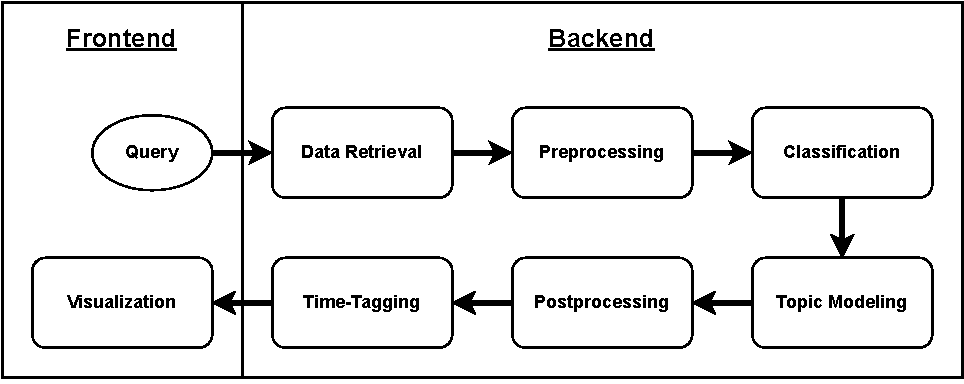
\includegraphics[width=\linewidth]{img/system.pdf}
\caption{Schematic Overview of the System's Data Processing Pipeline.}
\label{fig:archi}
\end{figure}

\subsubsection{Classification}
Our classifier was implemented using a DistilRoBERTa\footnote{\url{https://huggingface.co/distilroberta-base}} model, which was fine-tuned by appending a feed-forward network to the output. DistilRoBERTa is a smaller, faster version of the renowned RoBERTa language model \cite{roberta}, trained to preserve its performance on downstream tasks. It was chosen over the larger RoBERTa model because our system requires real-time inference, where speed is critical. To further increase performance, the sequence length was reduced to 50 tokens. Considering that the model only processes one sentence at a time, and given that the average sentence length in our dataset is 20 words, this is sufficient.
The outputs from the DistilRoBERTa model undergo mean pooling to produce a 768-dimensional vector, which is then fed into our fine-tuning feed-forward network.

\paragraph{Training Insights}
We fine-tuned the network on our dataset over the course of 14 epochs with the following configurations:
\begin{itemize}
    \item Batch size: 8
    \item Learning rate: 1.5e-6
    \item Warmup: 0.2
    \item Weight decay: 0.001
\end{itemize}

\paragraph{Validation Insights}
We employed 10-fold cross-validation to obtain performance estimates for the model. The following metrics show the average scores we achieved:
\begin{itemize}
    \item Accuracy: 0.965
    \item Precision: 0.953
    \item Recall: 0.98
    \item F1-score: 0.97
    \item AUC-ROC: 0.964
\end{itemize}
\paragraph{Inference}
The preprocessed sentences are fed into the fully trained model, which outputs a score between 0 and 1, indicating the probability that the sentence is future-related. Sentences with a probability above 0.9 are considered positives and are forwarded to the topic modeling step. %To enable active learning, all sentences are stored together with their confidence scores, subsequently manually labeled and inserted into the training dataset.

\subsubsection{Topic Modeling}
To present the user with sentences assigned to topics, we perform topic modeling using BERTopic\footnote{\url{https://maartengr.github.io/BERTopic/index.html}}, a system that extracts topics from text documents by embedding them in a high-dimensional space using SBERT\footnote{\url{https://www.sbert.net/}} and then clustering the embeddings by similarity.
It also extracts representative keywords from the topics, which are used as topic headings. We configured BERTopic to perform dimensionality reduction with UMAP\footnote{\url{https://umap-learn.readthedocs.io/en/latest/}} and clustering with HDBSCAN\footnote{\url{https://hdbscan.readthedocs.io/en/latest/}}.

\subsubsection{Postprocessing}
To improve the quality of topic modeling results and rank sentences based on their relevance, we postprocess the results in two ways.
First, we remove outliers from topics by matching the topic keywords against the words in each sentence. If a sentence contains fewer than three topic keywords, it is removed from the dataset.
The next step eliminates redundancy within a topic and evaluates the relevance of each sentence. Using the previously generated SBERT sentence embeddings from the topic modeling step, we calculate the cosine similarity between all sentence pairs within the same topic. When two sentences have a cosine similarity above 0.8, they are considered duplicates. The shorter sentence is discarded, and the duplicate count of the longer sentence is incremented. This duplicate count serves as a measure of sentence relevance. The greater the number of duplicates, the more frequently the sentence appeared in news articles and the more relevant it might be.

\subsubsection{Time-Tagging}
To create a timeline, we need to map sentences to concrete dates. This requires the identification and resolution of temporal expressions in the sentences. The SUTime\footnote{\url{https://nlp.stanford.edu/software/sutime.shtml}} time-tagger was employed for this purpose. It detects temporal information and resolves it to the referenced date, incorporating the article's publication date.
Some rules had to be added to ensure that all temporal expressions are mapped to dates, such as mapping \textit{'Summer'} to \textit{'07.08'}.
While the tagger generally performs well, there are some problems with ambiguous references like \textit{'On Tuesday, he revealed his decision, which will become official soon'}.
The time-tagger maps \textit{"on Tuesday"} to the coming Tuesday, which is in the future, even though the sentence is referring to a past event. This is a known limitation of SUTime, which is mitigated by simply discarding extracted temporal expressions that reference weekdays.

\subsection{Demonstration System}
The system was implemented as a web app with a Vue.js\footnote{\url{https://vuejs.org/}} frontend and a Django\footnote{\url{https://www.djangoproject.com/}} backend. It can be accessed with a standard browser at the following URL: \textit{\url{http://chronicle2050.regevson.com}}. Due to the workflow taking a significant amount of time, the whole process is executed multiple times, each time downloading new articles, classifying them and then clustering them together with the previously extracted sentences. When new results are ready, a button appears, which lets the user give permission to load in the updated data.

\subsubsection{Settings}
Upon entry, the website shows a settings panel that provides the user with some adjustable configurations. Here, decisions about whether updates should be automatic or manual can be made. There's also the possibility to specify the quantity of articles and their time frame. A text field prompts users to specify an entity for exploration.

%\subsubsection{Statistics}
%A statistics section is available, putting the data in numbers. Here, users can see the fraction of sentences that contain temporal expressions, get insights into the number of topic clusters, and see the average number of sentences per cluster.

\subsubsection{Timeline}
The website's core component is the timeline visualization. As shown in Figure \ref{fig:ui} (left), the y-axis shows the different topics, whereas the x-axis displays future dates referenced by the sentences. A data point on the timeline represents a collection of sentences belonging to the same topic, that all reference the same date. This collection of sentences is revealed when hovering over the datapoint in the form of a tooltip section. They are ranked according to their relevance score, which is also displayed next to each sentence. There is also an option to delve into the full article for more context, by simply clicking on a sentence. The data point itself has a color assigned to it, representing the relevance of the sentences it contains, with red colors indicating higher relevance.

\subsubsection{Word Cloud}
Complementing the timeline, the word cloud visualization, depicted in Figure \ref{fig:ui} (right), provides the user with sentences that do not contain any temporal expressions. Each topic is represented as a cloud, whose size corresponds to the mean relevance of the contained sentences. On interaction, these clouds unfold to reveal the associated sentences, again along with their relevance scores and with links to their origin articles.

\section{Evaluation}
To assess the effectiveness of our system, we developed a six-task exercise and presented it to six different users. Each user had to complete the exercise with one of three entities. These tasks were designed to examine the timeline and word cloud components. The tasks included: 1) summarizing the entity's future outlook, 2) determining which topic and date have the highest/lowest relevance and analyzing the overall ranking, 4) engaging with the timeline to find incorrectly resolved temporal expressions, 5) summarizing the content of the most relevant word cloud, 6) examining the word clouds for duplicate content and 7) examining both components for sentences without future-related content.

The users provided lengthy summaries, implying a wide range of predictions for upcoming years. The color-coding of datapoints managed to successfully convey relevance, but users noticed that nearer predictions were generally marked as more relevant, while key distant predictions often had lower relevance scores. Some users found this to be a problem, as distant events are often more significant and require more time to unfold. The time-tagging was generally accurate but struggled with some past predictions like \textit{"In 2019, he correctly predicted that a pandemic would occur by the end of the year"}. This is because the tagger resolves temporal expressions relative to the parent article's publishing date, and does not understand that \textit{"in 2019"} should be the anchor date. Some users found similar sentences in the same cluster, but the information they provided was slightly different. This provided additional context, which was well-received.

Overall, the system received strong approval from its users. On a five-star scale, the topic and classification quality received an average rating of 4 stars, while time-tagging quality received 3 stars. The ranking was evaluated at 3.5 stars, and the visualization received a 4.5-star average. Users were particularly satisfied with the ability of the system to provide information about an entity's future plans, events, and decisions. However, the biggest critique was the system's speed, especially the time it takes to retrieve the initial results. This should be kept for future work.

%\vfill\eject

\section{Conclusions}
By developing a multi-source dataset of 6,800 labeled sentences, we fine-tuned a DistilRoBERTa model to identify future references.  We then used BERTopic for topic modeling and SUTime for time-tagging to extract topics from the data and detect and resolve temporal expressions. A dedicated postprocessing step improved cluster quality and ranked sentences according to their relevance. We also designed an intuitive interface that presents the results with an interactive timeline and word clouds. A user study confirmed the system's ability to offer a detailed overview of the future, while also highlighting potential areas for improvement, especially speed.



%%
%% The next two lines define the bibliography style to be used, and
%% the bibliography file.
\bibliographystyle{ACM-Reference-Format}
\bibliography{sample-base}

\end{document}
\endinput
%%
%% End of file `sample-sigconf.tex'.